\documentclass[twoside,11pt]{article}\usepackage[]{graphicx}\usepackage[]{xcolor}
% maxwidth is the original width if it is less than linewidth
% otherwise use linewidth (to make sure the graphics do not exceed the margin)
\makeatletter
\def\maxwidth{ %
  \ifdim\Gin@nat@width>\linewidth
    \linewidth
  \else
    \Gin@nat@width
  \fi
}
\makeatother

\definecolor{fgcolor}{rgb}{0.345, 0.345, 0.345}
\newcommand{\hlnum}[1]{\textcolor[rgb]{0.686,0.059,0.569}{#1}}%
\newcommand{\hlstr}[1]{\textcolor[rgb]{0.192,0.494,0.8}{#1}}%
\newcommand{\hlcom}[1]{\textcolor[rgb]{0.678,0.584,0.686}{\textit{#1}}}%
\newcommand{\hlopt}[1]{\textcolor[rgb]{0,0,0}{#1}}%
\newcommand{\hlstd}[1]{\textcolor[rgb]{0.345,0.345,0.345}{#1}}%
\newcommand{\hlkwa}[1]{\textcolor[rgb]{0.161,0.373,0.58}{\textbf{#1}}}%
\newcommand{\hlkwb}[1]{\textcolor[rgb]{0.69,0.353,0.396}{#1}}%
\newcommand{\hlkwc}[1]{\textcolor[rgb]{0.333,0.667,0.333}{#1}}%
\newcommand{\hlkwd}[1]{\textcolor[rgb]{0.737,0.353,0.396}{\textbf{#1}}}%
\let\hlipl\hlkwb

\usepackage{framed}
\makeatletter
\newenvironment{kframe}{%
 \def\at@end@of@kframe{}%
 \ifinner\ifhmode%
  \def\at@end@of@kframe{\end{minipage}}%
  \begin{minipage}{\columnwidth}%
 \fi\fi%
 \def\FrameCommand##1{\hskip\@totalleftmargin \hskip-\fboxsep
 \colorbox{shadecolor}{##1}\hskip-\fboxsep
     % There is no \\@totalrightmargin, so:
     \hskip-\linewidth \hskip-\@totalleftmargin \hskip\columnwidth}%
 \MakeFramed {\advance\hsize-\width
   \@totalleftmargin\z@ \linewidth\hsize
   \@setminipage}}%
 {\par\unskip\endMakeFramed%
 \at@end@of@kframe}
\makeatother

\definecolor{shadecolor}{rgb}{.97, .97, .97}
\definecolor{messagecolor}{rgb}{0, 0, 0}
\definecolor{warningcolor}{rgb}{1, 0, 1}
\definecolor{errorcolor}{rgb}{1, 0, 0}
\newenvironment{knitrout}{}{} % an empty environment to be redefined in TeX

\usepackage{alltt}

% Any additional packages needed should be included after jmlr2e.
% Note that jmlr2e.sty includes epsfig, amssymb, natbib and graphicx,
% and defines many common macros, such as 'proof' and 'example'.
%
% It also sets the bibliographystyle to plainnat; for more information on
% natbib citation styles, see the natbib documentation, a copy of which
% is archived at http://www.jmlr.org/format/natbib.pdf

% Available options for package jmlr2e are:
%
%   - abbrvbib : use abbrvnat for the bibliography style
%   - nohyperref : do not load the hyperref package
%   - preprint : remove JMLR specific information from the template,
%         useful for example for posting to preprint servers.
%
% Example of using the package with custom options:
%
% \usepackage[abbrvbib, preprint]{jmlr2e}

\usepackage{jmlr2e}
% extra packages
\usepackage{longtable}
\usepackage{colortbl}
\usepackage{amsmath}
\usepackage{booktabs}
\usepackage{caption}
\usepackage{hyperref}
\hypersetup{hidelinks}
\usepackage{geometry}
\usepackage{pdflscape}
\usepackage{bm}

\definecolor{lightgray}{rgb}{0.83, 0.83, 0.83}

% Definitions of handy macros can go here

\newcommand{\dataset}{{\cal D}}
\newcommand{\fracpartial}[2]{\frac{\partial #1}{\partial  #2}}
\newcommand{\ie}{that is}
\newcommand{\eg}{for example}
\newcommand{\cstat}{\widehat{\text{C}}(t)}
\newcommand{\bstat}{\widehat{\text{BS}}(t)}
\newcommand{\bsbar}{\mathcal{\widehat{BS}}(t_1, t_2)}
\newcommand{\bskap}{\mathcal{\widehat{BS}}_0(t_1, t_2)}

\newcommand{\ntrain}{N_{\text{train}}}
\newcommand{\ntest}{N_{\text{test}}}


% Heading arguments are {volume}{year}{pages}{date submitted}{date published}{paper id}{author-full-names}

\jmlrheading{1}{2000}{1-48}{4/00}{10/00}{meila00a}{Marina Meil\u{a} and Michael I. Jordan}

% Short headings should be running head and authors last names

\ShortHeadings{Accelerated oblique random survival forests}{Jaeger et al}
\firstpageno{1}
\IfFileExists{upquote.sty}{\usepackage{upquote}}{}
\begin{document}

\title{Accelerated oblique random survival forests}

\author{\name Byron C. Jaeger \email bjaeger@wakehealth.edu \\
       \addr Department of Biostatistics and Data Science\\
       Wake Forest University School of Medicine\\
       Winston-Salem, NC 27157, USA
       \AND
       \name Sawyer Welden \email swelden@wakehealth.edu \\
       \addr Department of Biostatistics and Data Science\\
       Wake Forest University School of Medicine\\
       Winston-Salem, NC 27157, USA
       \AND
       \name Kristin Lenoir \email klenoir@wakehealth.edu \\
       \addr Department of Biostatistics and Data Science\\
       Wake Forest University School of Medicine\\
       Winston-Salem, NC 27157, USA
       \AND
       \name Jaime L Speiser \email jspeiser@wakehealth.edu \\
       \addr Department of Biostatistics and Data Science\\
       Wake Forest University School of Medicine\\
       Winston-Salem, NC 27157, USA
       \AND
       \name Matthew Segar \email Matthew.Segar@UTSouthwestern.edu \\
       \addr Division of Cardiology, Department of Internal Medicine, \\
       University of Texas Southwestern Medical Center, Dallas
       \AND
       \name Nicholas M. Pajewski \email npajewsk@wakehealth.edu \\
       \addr Department of Biostatistics and Data Science\\
       Wake Forest University School of Medicine\\
       Winston-Salem, NC 27157, USA}

\editor{TBD}

\maketitle



\newpage

\begin{abstract}%   <- trailing '%' for backward compatibility of .sty file

The oblique random survival forest (ORSF) is an ensemble method for supervised learning that extends the random survival forest (RSF). Trees in the ORSF are grown using linear combinations of variables to create branches in the tree, whereas in the RSF a single variable is used. ORSF ensembles often have higher prediction accuracy than RSF ensembles, but the additional computational overhead of fitting ORSF ensembles limits their scope of application. In addition, few methods have been developed for interpretation of ORSF ensembles. In this article, we introduce and evaluate methods to accelerate the ORSF (\ie, reduce computational overhead) and compute the importance of individual variables in the ORSF We show that our strategy to accelerate the ORSF is up to 500 times faster than existing software for ORSFs (the \texttt{obliqueRSF} R package), and that prediction accuracy of the accelerated ORSF is equivalent or superior to that of existing ORSF methods. We estimate importance of variables for the ORSF by negating each coefficient used for the given variable in linear combinations, and then computing the reduction in out-of-bag accuracy. We show with simulation that  `negation importance' can discriminate between signal and noise variables, and it outperforms several state-of-the-art variable importance techniques in this task when there is correlation among predictors.

\end{abstract}

\begin{keywords}
  Random Forests, Survival, Efficient, Variable Importance
\end{keywords}

\section{Introduction}

Risk prediction can reduce the burden of disease by educating patients and providers and guiding strategies to prevent and treat disease in a wide range of medical domains \citep{moons2012riskII, moons2012riskI}. The random survival forest (RSF), a supervised learning algorithm that can engage with censored outcomes, is frequently used for risk prediction. Notable characteristics of the RSF include uniform convergence of its ensemble survival function to the true population survival function when the predictor space is discrete \citep{ishwaran2010consistency}. In addition, software implementing the RSF is freely available, extremely efficient, and full of tools to interpret and explain the RSF \citep{randomForestSRC, ranger, hothorn2010party}. However, there remains considerable potential to improve the RSF in risk prediction tasks where training samples are not large enough to guarantee asymptotic properties or predictor spaces are non-discrete (\ie, predictors are continuous).

RSFs may be axis based or oblique. The axis based RSF uses a single predictor whereas the oblique RSF uses a linear combination of predictors to create branches in trees. While axis based decision boundaries are always perpendicular to the axis of the relevant predictor, linear combinations of predictors create oblique decision boundaries that are neither parallel nor perpendicular to axes of their contributing predictors. Prior work has found the oblique RSF has higher prediction accuracy than the axis based RSF in general benchmarks \citep{jaeger2019oblique} and that oblique splitting is particularly effective when predictors are continuous \citep{menze2011oblique}. However, existing methods to implement oblique splitting typically use fully trained models in each non-leaf node to identify linear combinations of predictors, exponentially increasing the number of operations required for the oblique RSF versus its axis based counterpart. In addition, standard methods to estimate variable importance (VI) in the RSF are less effective in the oblique RSF, and few methods have been introduced to estimate VI specifically for the oblique RSF.

The aim of this article is to improve the computational efficiency and interpretability of the oblique RSF. In a general benchmark experiment including YYYY risk prediction tasks, we show that oblique RSFs with partially trained models have equivalent or superior prediction accuracy and are orders of magnitude more efficient than oblique RSFs with fully trained models in non-leaf nodes. We introduce a method to estimate VI for oblique RSFs and compare its ability to discriminate between signal and noise variables versus standard and state-of-the-art methods. All methods proposed in this article are available in the \texttt{aorsf} R Package.

\section{Related work}

\subsection{Axis-based and oblique random forests}

After \citet{breiman2001random} introduced the axis-based and oblique random forest (RF), numerous methods were developed to grow oblique RFs for classification or regression tasks \citep{menze2011oblique, zhang2014oblique, rainforth2015canonical, zhu2015reinforcement, poona2016investigating, qiu2017oblique, tomita2020sparse, katuwal2020heterogeneous}. However, oblique splitting approaches for classification or regression may not generalize to survival tasks \citep[\eg, see][Section~4.5.1]{zhu2013tree}, and most research involving the RSF has focused on forests with axis-based trees \citep{wang2017selective}.

Building on prior research for bagging survival trees \citep{hothorn2004bagging}, \citet{hothorn2006unbiased} developed an axis-based RSF in their framework for unbiased recursive partitioning, more commonly referred to as the conditional inference forest (CIF). \citet{zhou2016random} developed a rotation forest based on the CIF and \citet{wang2017random} developed a method for extending the predictor space of the CIF. \citet{ishwaran2008random} developed an axis-based RSF with strict adherence to the rules for growing trees proposed in \citet{breiman2001random}. \citet{jaeger2019oblique} developed the oblique RSF following the bootstrapping approach described in Breiman's original RF and incorporating early stopping rules from the CIF.

\subsection{Variable importance}

\citet{breiman2001random} introduced permutation VI, defined for each predictor as the difference in a RF's estimated generalization error before versus after the predictor's values are randomly permuted. \citet{strobl2007bias} identified bias in permutation VI driven by variable selection bias and effects induced by bootstrap sampling, and proposed an unbiased permutation VI based on unbiased recursive partitioning (see \citet{hothorn2006unbiased}). \citet{menze2011oblique} introduced an approach to estimate VI for oblique RFs that computes an analysis of variance (ANOVA) table in non-leaf nodes to obtain p-values for each predictor contributing to the node. The ANOVA VI\footnote{\citet{menze2011oblique} name their method `oblique RF VI', but we use the name `ANOVA VI' in this article to avoid confusing Menze's approach with other approaches to estimate VI for oblique RFs.} is then defined for each predictor as the number of times a p-value associated with the predictor is $\leq 0.01$ while growing a forest. \citet{lundberg2017unified} introduced a method to estimate VI using SHapley Additive exPlanation (SHAP) values, which estimate the contribution of a predictor to a model's prediction for a given observation. SHAP VI is computed for each predictor by taking the mean absolute value of SHAP values for that predictor across all observations in a given set.

% Several supervised learning algorithms can develop prediction functions for right-censored time-to-event outcomes, henceforth referred to as survival outcomes. \cite{ishwaran2008random} developed the RF for survival, an extension of the RF for regression and classification developed by \citet{breiman2001random}. Fast algorithms to fit the RF for survival are available in the \texttt{randomForestSRC} R package \citep{randomForestSRC}. A similar implementation of the RF for survival can be found in the \texttt{ranger} R package \citep{ranger}, which is particularly suited for high dimensional data. The RF for survival can also be fit using unbiased recursive partitioning \citep{cif} via the \texttt{party} R package \citep{hothorn2010party}.

\section{Novel techniques for oblique random survival forests}

Consider the usual framework for survival analysis with training data $$\dataset_{\text{train}} = \left\{ (T_i, \delta_i, \bm{x}_{i}) \right\}_{i=1}^{N_{\text{train}}}.$$ Here, $T_i$ is the event time if $\delta_i=1$ and last point of contact if $\delta_i=0$, and $\bm{x}_i$ is a vector of predictors values. Assuming there are no ties, let $t_1 < \, \ldots \, < t_m$ denote the $m$ unique event times in $\dataset_{\text{train}}$.

\subsection{Partial training at non-leaf nodes}

We propose to identify linear combinations of predictor variables in non-leaf nodes by applying Newton Raphson scoring to the partial likelihood function of the Cox regression model:
\begin{equation}\label{eqn:cox-partial-likelihood}
L(\bm\beta) = \prod_{i=1}^m \frac{e^{\bm{x}_{j(i)}^T \bm\beta}}{\sum_{j \in R_i} e^{\bm{x}_j^T \bm\beta}},
\end{equation}
where $R_i$ is the set of indices, $j$, with $T_j \geq t_i$ (i.e., those still at risk at time $t_i$), and $j(i)$ is the index of the observation for which an event occurred at time $t_i$. The \texttt{survival} package includes documentation that outlines how to complete this estimation procedure efficiently \citep[see][exact.nw]{therneau_survival_2022}. Briefly, a vector of estimated regression coefficients, $\hat{\beta}$, is updated in each step of the procedure based on its first derivative, $U(\hat{\beta})$, and second derivative, $H(\hat{\beta})$:
$$ \hat{\beta}^{k+1} =  \hat{\beta}^{k} + U(\hat{\beta} = \hat{\beta}^{k})\, H^{-1}(\hat{\beta} = \hat{\beta}^{k}) $$
It is vital to cycle through iterations until a convergence threshold is met for statistical inference, but it is only necessary to complete one iteration to identify coefficients for a linear combination of predictors. \citet{jaeger2019oblique} identified linear combinations using penalized regression models, which supply more flexible solutions for $\hat{\beta}$ at the cost of greater computational demand.

\subsection{Negation variable importance}

Negation VI is similar to permutation VI in that it measures how much a model’s prediction error increases when a variable’s role in the model is de-stabilized. More specifically, negation VI measures the increase in an oblique RF's prediction error after flipping the sign of all coefficients linked to a variable (\ie, negating them). As the magnitude of a coefficient increases, so does the probability that negating it will change the oblique RF's predictions. Since the coefficients in each non-leaf node of an oblique RFs are adjusted for the accompanying predictors, negation VI may provide better estimation of VI in the presence of correlated variables compared to standard VI techniques. Although the current article focuses on oblique RSFs, negation VI can be applied to any oblique RF.

\section{Numeric experiments}

\subsection{Benchmark of prediction accuracy}

\subsubsection{Learners}

We consider four classes of learners: RFs, boosting ensembles, regression models, and neural networks (Table \ref{table:learners}). For RF learners, the number of observations required in terminal nodes was fixed at 10, the number of randomly selected predictors was the square root of the total number of predictors rounded to the nearest integer, and the number of trees in the ensemble was 500. For boosting, regression, and neural network learners, nested cross-validation was applied to tune each model, \ie, assess multiple possible values for relevant model parameters and use the values that optimize the model's estimated prediction accuracy. Specifically, tuning for boosting models included identifying the number of steps to complete. For regression models, tuning was used to identify the magnitude of penalization. For neural networks, the number and density of layers was tuned.

\newgeometry{margin=1cm} % modify this if you need even more space
\begin{landscape}

\begin{table}[h!]
\centering
\begin{tabular}{p{2cm} | p{3cm} p{4cm} p{12cm}}
 \hline
 Learner Class & Software & Learners & Description \\ [0.5ex]
 \hline\hline
 \multicolumn{3}{l}{\textit{Random Survival Forests}}\\
 \hline\hline

 Axis based &

 \href{https://www.randomforestsrc.org/index.html}{\texttt{RandomForestSRC}} \newline
 \href{https://CRAN.R-project.org/package=ranger}{\texttt{ranger}} \newline
 \href{http://party.r-forge.r-project.org/}{\texttt{party}} \newline
 \href{https://github.com/whcsu/rotsf}{\texttt{rotsf}} \newline
 \href{https://github.com/whcsu/rsfse}{\texttt{rsfse}} &

 \texttt{rsf-standard} \newline
 \texttt{rsf-extratrees} \newline
 \texttt{cif-standard} \newline
 \texttt{cif-rotate} \newline
 \texttt{cif-spacextend} &

 \texttt{rsf-standard} grows survival trees following Leo Breiman's original random forest algorithm with variables and cut-points selected to maximize a log-rank statistic. \texttt{rsf-extratrees} grows survival trees with randomly selected features and cut-points. \texttt{cif-standard} uses the framework of conditional inference to grow survival trees. \texttt{cif-rotate} extends \texttt{cif-standard} by applying principal component analysis to random subsets of data prior to growing each survival tree. \texttt{cif-spacextend} derives new predictors for each tree in the ensemble, separately. \\ \hline


 Oblique &


 \href{https://CRAN.R-project.org/package=obliqueRSF}{\texttt{obliqueRSF}} \newline
 \href{https://bcjaeger.github.io/aorsf/}{\texttt{aorsf}} &

 \texttt{obliqueRSF-net} \newline
 \texttt{aorsf-net} \newline
 \texttt{aorsf-fast} \newline
 \texttt{aorsf-cph} \newline
 \texttt{aorsf-extratrees} &


 Oblique survival trees following Leo Breiman's random forest algorithm. Linear combinations of inputs are derived using \texttt{glmnet} in \texttt{obliqueRSF-net} and \texttt{aorsf-net}, using Newton Raphson scoring for the Cox partial likelihood function in \texttt{aorsf-fast} and \texttt{aorsf-cph}, and chosen randomly from a uniform distribution in \texttt{aorsf-extratrees}. Cut-points are selected to maximize a log-rank statistic. \\

 \hline\hline
 \multicolumn{3}{l}{\textit{Boosting ensembles}}\\
 \hline\hline

 Trees &

 \href{https://xgboost.readthedocs.io/en/stable/#}{\texttt{xgboost}} &

 \texttt{xgboost-cox} \newline
 \texttt{xgboost-aft} &

 \texttt{xgboost-cox} maximizes the Cox partial likelihood function, whereas \texttt{xgboost-aft} maximizes the accelerated failure time likelihood function. Nested cross validation (5 folds) is applied to tune the number of trees grown, the minimum number of observations in a leaf node was 10, the maximum depth of trees was 6, and $\sqrt{p}$ variables were considered randomly for each tree split, where $p$ is the total number of predictors. \\
 \hline\hline
 \multicolumn{3}{l}{\textit{Regression models}}\\
 \hline\hline
 Cox Net & \texttt{glmnet} & \texttt{glmnet-cox} & The Cox proportional hazards model is fit using an elastic net penalty. Nested cross validation (5 folds) is applied to tune penalty terms.\\
 \hline\hline
 \multicolumn{3}{l}{\textit{Neural networks}}\\
 \hline\hline
 Cox Time & \href{https://raphaels1.github.io/survivalmodels/}{\texttt{survivalmodels}} & \texttt{nn-cox} & A neural network based on the proportional hazards model with time-varying effects. Nested cross-validation was applied to select the number of layers (from 1 to 8), the number of nodes in each layer (from $\sqrt{p}$/2 to $\sqrt{p}$), and the number of epochs to complete (up to 500). A drop-out rate of 10\% was applied during training.   \\
 \hline
\end{tabular}
\caption{Learning algorithms assessed in numeric studies}
\label{table:learners}
\end{table}

\end{landscape}
\restoregeometry


\subsubsection{Evaluation of prediction accuracy} \label{sec:prediction_accuracy}

Our primary metric for evaluating the accuracy of predicted risk is the integrated and scaled Brier score \citep{graf1999assessment}. For observation $i$ in the testing data, let $\widehat{S}(t \mid \bm{x}_i)$ be the predicted probability of survival up to a given prediction horizon of $t > 0$ and let $\bm{x}_i$ be the vector of predictor values. Define \begin{align*}
\bstat = \frac{1}{\ntest} \sum_{i=1}^{\ntest} &\{ \widehat{S}(t \mid \bm{x}_i)^2 \cdot I(T_i \leq t, \delta_i = 1) \cdot \widehat{G}(T_i)^{-1} \\ &+ [1-\widehat{S}(t \mid \bm{x}_i)]^2 \cdot I(T_i > t) \cdot \widehat{G}(t)^{-1}\}
\end{align*} where $\widehat{G}(t)$ is the Kaplan-Meier estimate of the censoring distribution. As $\bstat$ is time dependent, integration over time provides a summary measure of performance over a range of plausible prediction horizons. The integrated $\bstat$ is defined as \begin{equation}
\bsbar = \frac{1}{t_2 - t_1}\int_{t_1}^{t_2} \widehat{\text{BS}}(t) dt.
\end{equation} In our results, $t_1$ and $t_2$ are the 25th and 75th percentile of event times, respectively. $\bsbar$, a sum of squared prediction errors, can be scaled to produce a measure of explained residual variation (\ie, an $R^2$ statistic) by computing \begin{equation}
R^2 = 1 - \frac{\bsbar}{\bskap}
\end{equation} where $\bskap$ is the integrated Brier score when a Kaplan-Meier estimate for survival based on the training data is used as the survival prediction function $\widehat{S}(t)$. We refer to this $R^2$ statistic as the index of prediction accuracy and we scale its values by 100 to avoid unnecessary leading zero's. For example, we present 25 if $R^2$ is 0.25 and present 10.2 if the difference between two $R^2$ is 0.102.

\subsubsection{Statistical analysis}

\subsubsection{Results}

\begin{knitrout}
\definecolor{shadecolor}{rgb}{0.969, 0.969, 0.969}\color{fgcolor}
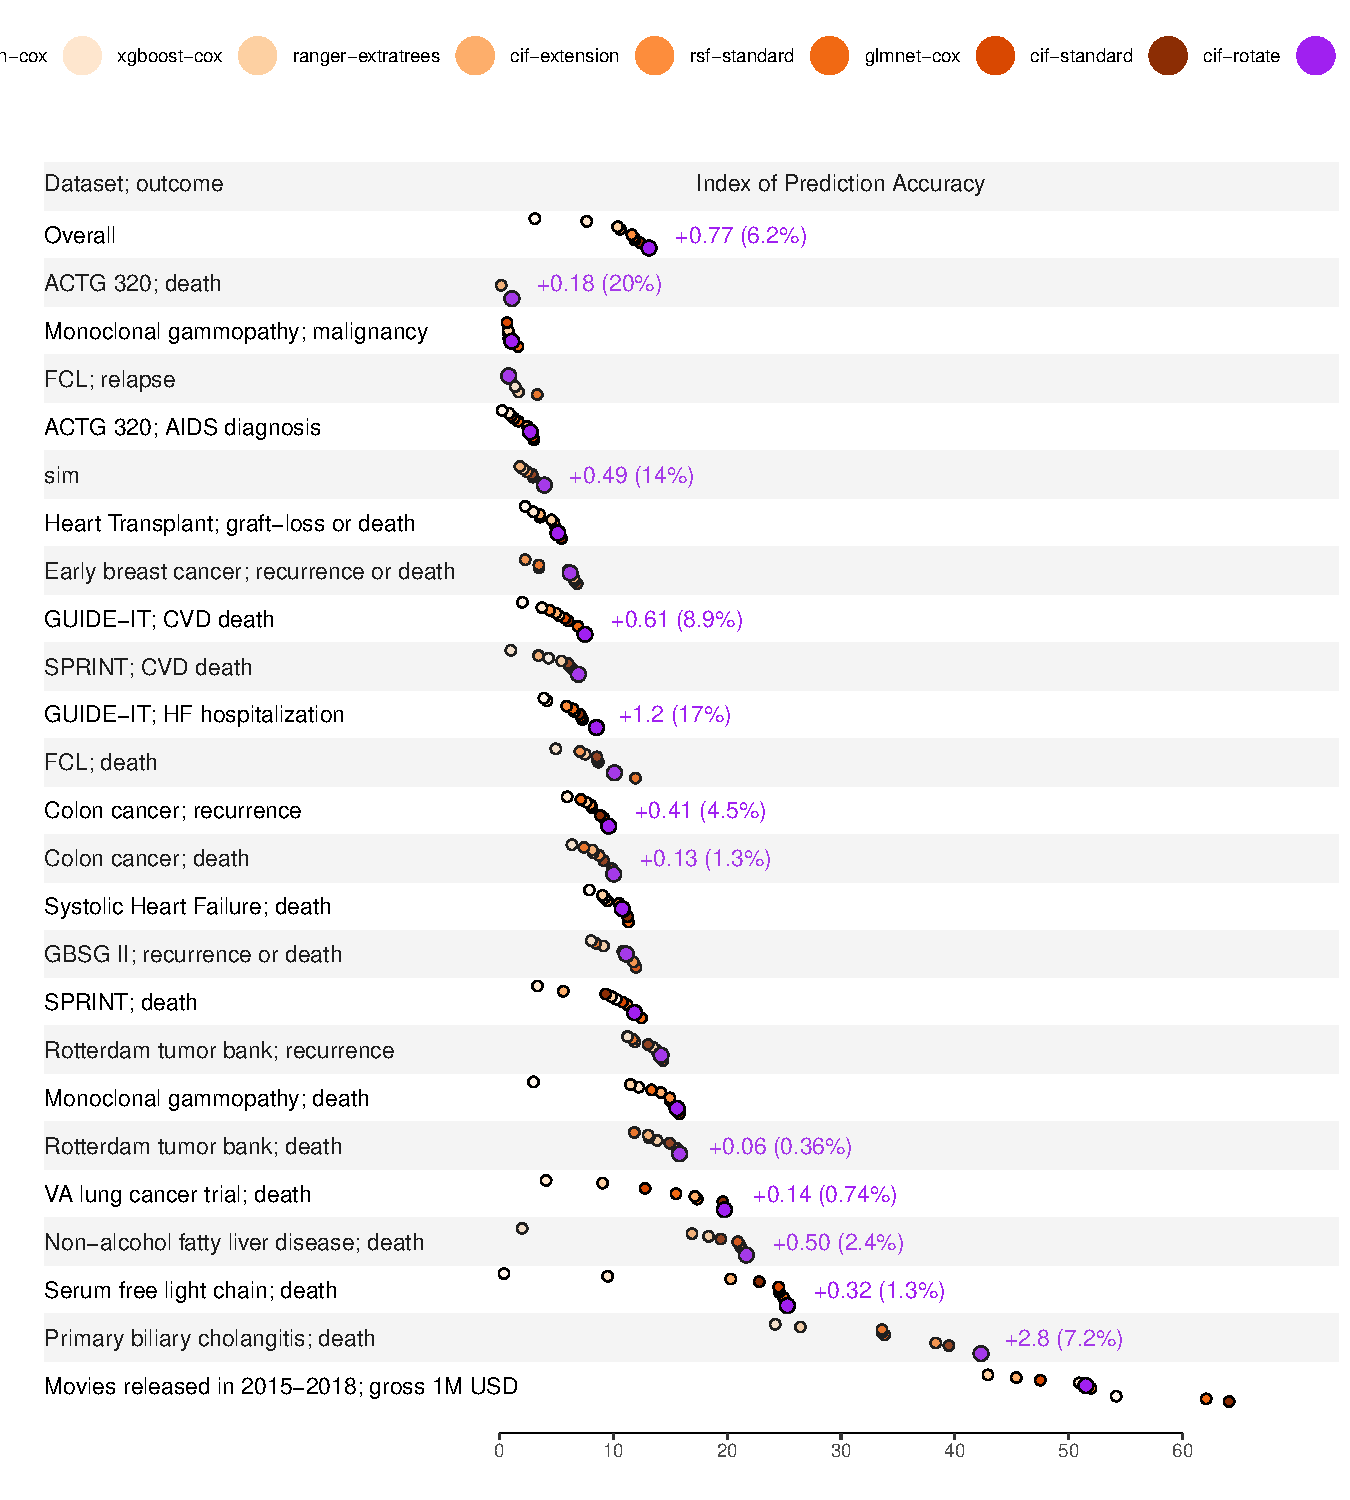
\includegraphics[width=\maxwidth]{figure/unnamed-chunk-2-1} 
\end{knitrout}


\begin{knitrout}
\definecolor{shadecolor}{rgb}{0.969, 0.969, 0.969}\color{fgcolor}
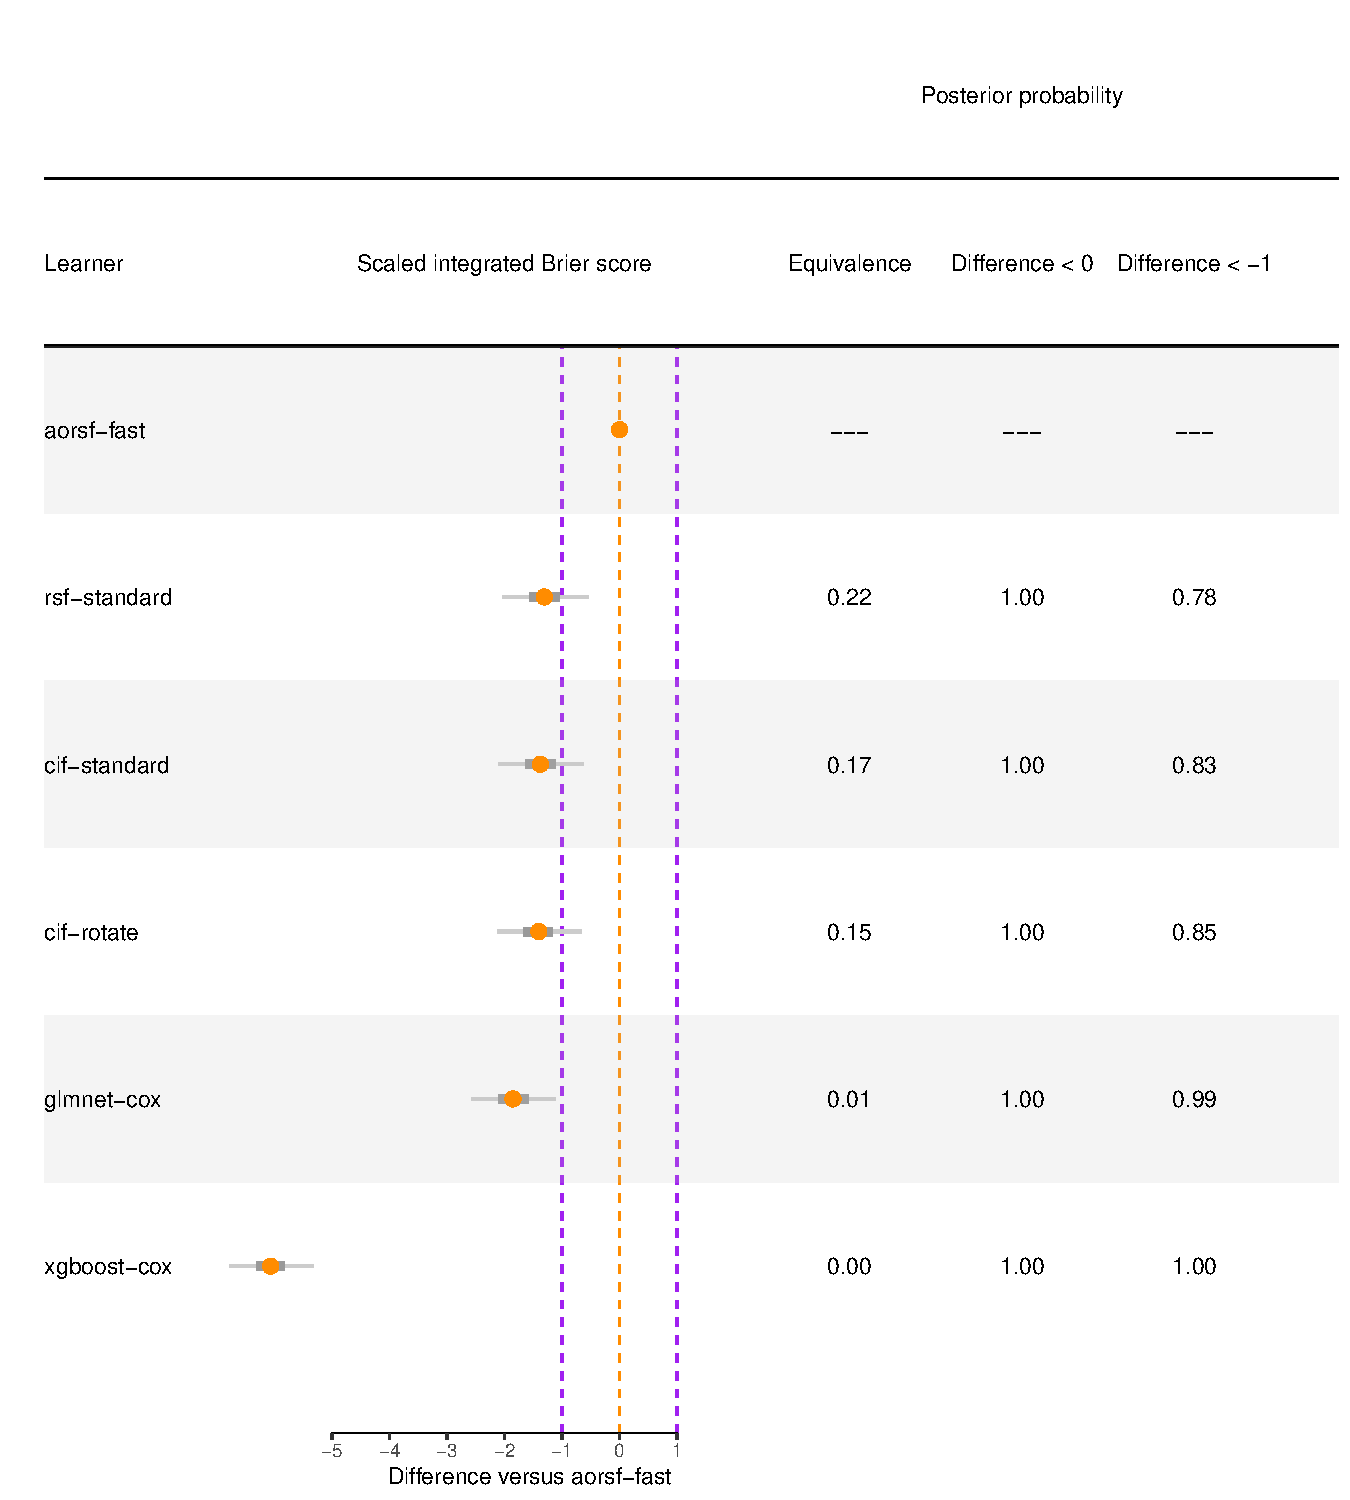
\includegraphics[width=\maxwidth]{figure/unnamed-chunk-3-1} 
\end{knitrout}

\subsection{Benchmark of variable selection}




% Acknowledgements should go at the end, before appendices and references

\acks{Research reported in this publication was supported by the Center for Biomedical Informatics, Wake Forest University School of Medicine}

% Manual newpage inserted to improve layout of sample file - not
% needed in general before appendices/bibliography.

\newpage

\appendix
\section*{Appendix A.}

\begin{knitrout}
\definecolor{shadecolor}{rgb}{0.969, 0.969, 0.969}\color{fgcolor}
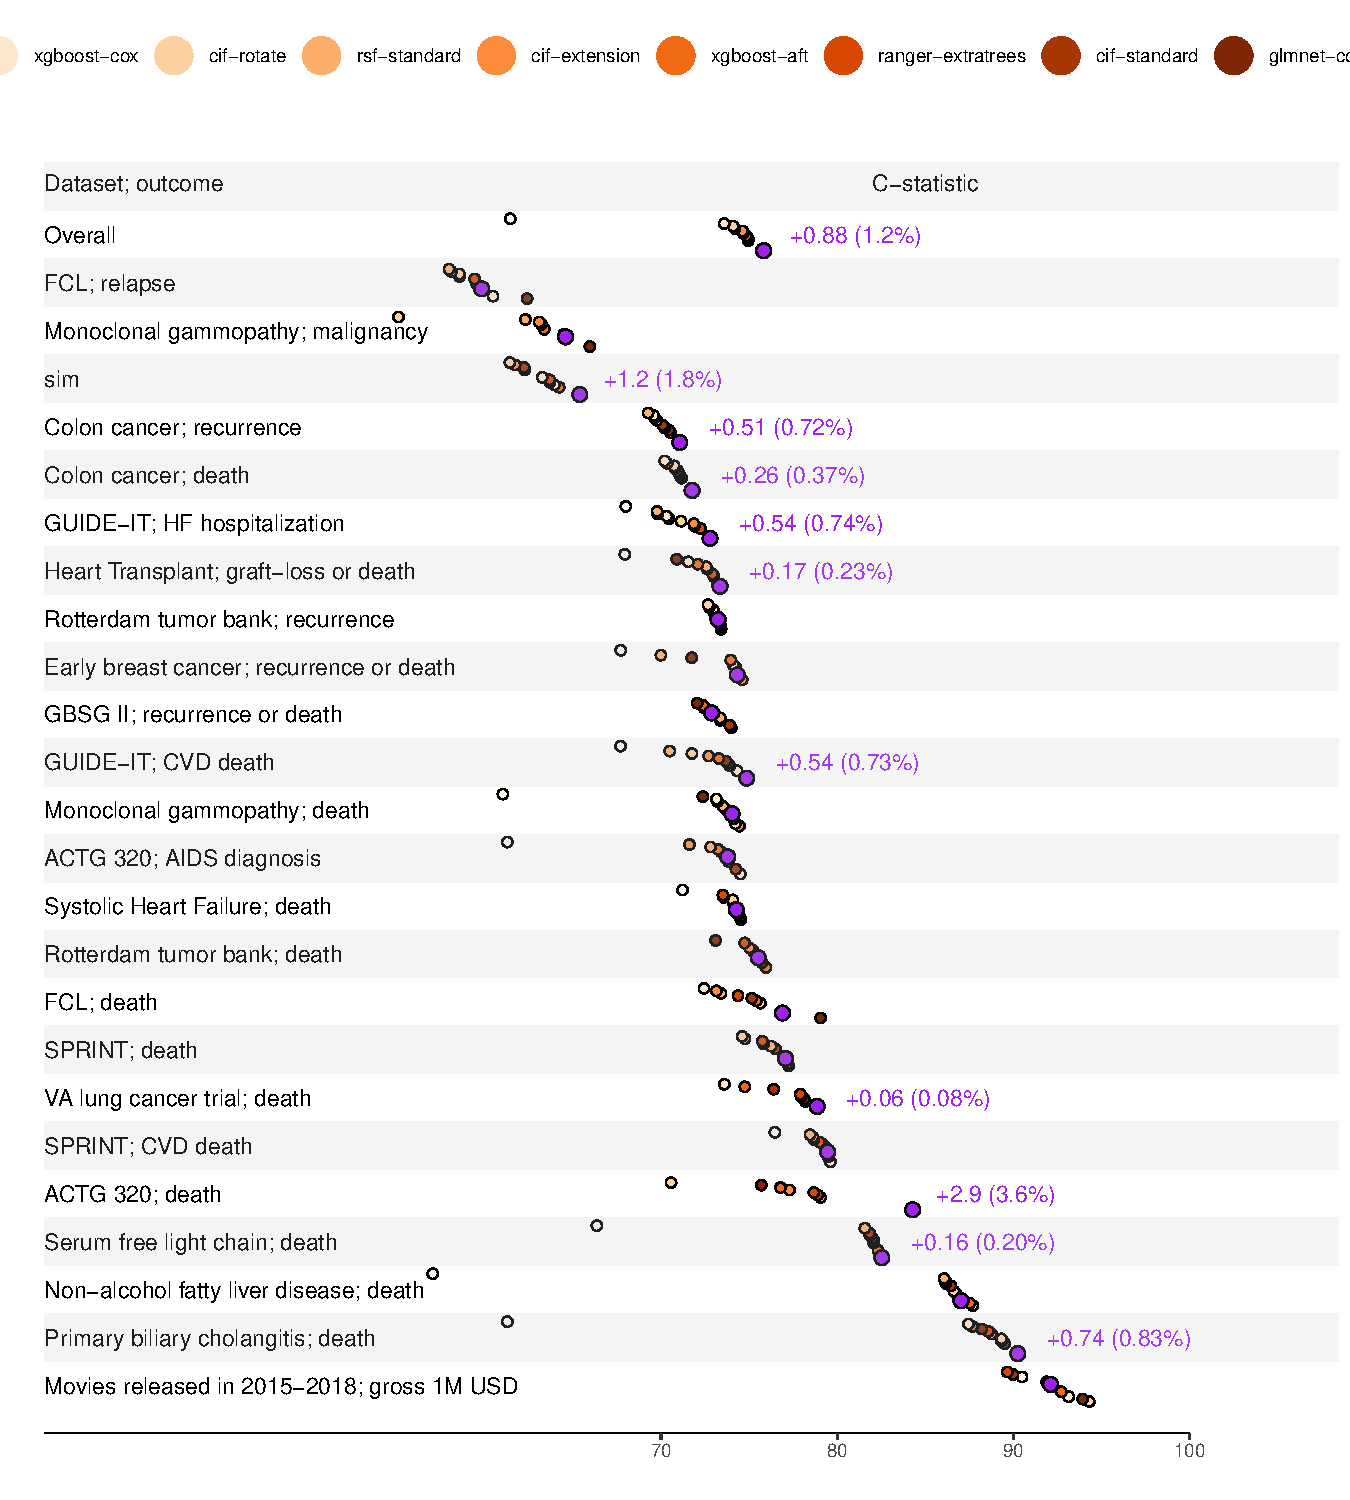
\includegraphics[width=\maxwidth]{figure/unnamed-chunk-4-1} 
\end{knitrout}

\newpage

\begin{knitrout}
\definecolor{shadecolor}{rgb}{0.969, 0.969, 0.969}\color{fgcolor}
\begin{longtable}{lcclccl}
\toprule
\multicolumn{3}{c}{ } & \multicolumn{4}{c}{Computing time, seconds} \\
\cmidrule(l{3pt}r{3pt}){4-7}
\multicolumn{1}{c}{ } & \multicolumn{2}{c}{Performance metric (SD)} & \multicolumn{2}{c}{Fit model} & \multicolumn{2}{c}{Predict risk} \\
\cmidrule(l{3pt}r{3pt}){2-3} \cmidrule(l{3pt}r{3pt}){4-5} \cmidrule(l{3pt}r{3pt}){6-7}
  & Scaled Brier & C-Statistic & Median & Ratio & Median & Ratio\\
\midrule
\endfirsthead
\multicolumn{7}{@{}l}{\textit{(continued)}}\\
\toprule
  & Scaled Brier & C-Statistic & Median & Ratio & Median & Ratio\\
\midrule
\endhead

\endfoot
\bottomrule
\endlastfoot
\addlinespace[0.3em]
\hline
\multicolumn{7}{l}{\textit{\textbf{Overall}}}\\
\hline
\hspace{1em}aorsf-cph & 0.133 (0.124) & 0.757 (0.079) & 0.830 & 2.74 & 0.070 & 0.980\\
\hspace{1em}aorsf-fast & 0.133 (0.124) & 0.757 (0.080) & 0.302 & 1.00 & 0.072 & 1.00\\
\hspace{1em}aorsf-net & 0.130 (0.127) & 0.755 (0.080) & 61.237 & 202.6 & 0.069 & 0.964\\
\hspace{1em}cif-rotate & 0.125 (0.145) & 0.741 (0.092) & 30.623 & 101.3 & 7.208 & 100.3\\
\hspace{1em}cif-standard & 0.120 (0.111) & 0.748 (0.079) & 2.035 & 6.73 & 5.128 & 71.3\\
\hspace{1em}glmnet-cox & 0.119 (0.139) & 0.748 (0.083) & 0.253 & 0.837 & 0.005 & 0.070\\
\hspace{1em}rsf-standard & 0.118 (0.128) & 0.741 (0.084) & 1.694 & 5.60 & 0.152 & 2.11\\
\hspace{1em}obliqueRSF-net & 0.117 (0.094) & 0.754 (0.080) & 328.883 & 1,087.9 & 26.636 & 370.5\\
\hspace{1em}cif-extension & 0.108 (0.108) & 0.746 (0.083) & 13.510 & 44.7 & 6.840 & 95.2\\
\hspace{1em}ranger-extratrees & 0.106 (0.097) & 0.748 (0.076) & 0.692 & 2.29 & 0.264 & 3.68\\
\hspace{1em}aorsf-random & 0.101 (0.092) & 0.735 (0.074) & 1.879 & 6.22 & 0.066 & 0.919\\
\hspace{1em}xgboost-cox & 0.077 (0.114) & 0.736 (0.095) & 3.833 & 12.7 & 0.005 & 0.070\\
\hspace{1em}nn-cox & 0.030 (0.118) & 0.610 (0.128) & 15.427 & 51.0 & 1.513 & 21.0\\
\hspace{1em}xgboost-aft & -3.68 (4.86) & 0.747 (0.082) & 13.182 & 43.6 & 0.008 & 0.117\\
\addlinespace[0.3em]
\hline
\multicolumn{7}{l}{\textit{\textbf{ACTG 320; AIDS diagnosis, n = 1151, p = 12}}}\\
\hline
\hspace{1em}aorsf-random & 0.028 (0.022) & 0.748 (0.038) & 0.637 & 4.19 & 0.040 & 1.06\\
\hspace{1em}ranger-extratrees & 0.028 (0.017) & 0.740 (0.036) & 0.061 & 0.404 & 0.184 & 4.81\\
\hspace{1em}obliqueRSF-net & 0.027 (0.022) & 0.746 (0.038) & 27.286 & 179.6 & 15.729 & 411.6\\
\hspace{1em}aorsf-cph & 0.025 (0.029) & 0.751 (0.042) & 0.450 & 2.97 & 0.034 & 0.891\\
\hspace{1em}cif-standard & 0.024 (0.031) & 0.744 (0.040) & 1.608 & 10.6 & 4.825 & 126.3\\
\hspace{1em}aorsf-fast & 0.024 (0.028) & 0.745 (0.044) & 0.152 & 1.00 & 0.038 & 1.00\\
\hspace{1em}cif-extension & 0.023 (0.015) & 0.722 (0.038) & 9.788 & 64.4 & 4.595 & 120.2\\
\hspace{1em}aorsf-net & 0.019 (0.034) & 0.745 (0.042) & 20.231 & 133.2 & 0.038 & 0.995\\
\hspace{1em}glmnet-cox & 0.016 (0.030) & 0.746 (0.037) & 0.183 & 1.21 & 0.002 & 0.053\\
\hspace{1em}rsf-standard & 0.005 (0.041) & 0.730 (0.042) & 0.235 & 1.55 & 0.071 & 1.85\\
\hspace{1em}cif-rotate & 0.004 (0.040) & 0.731 (0.038) & 15.089 & 99.3 & 4.246 & 111.1\\
\hspace{1em}xgboost-cox & 0.000 (0.044) & 0.751 (0.033) & 3.655 & 24.1 & 0.003 & 0.079\\
\hspace{1em}nn-cox & 0.000 (0.013) & 0.574 (0.117) & 12.345 & 81.3 & 0.639 & 16.7\\
\hspace{1em}xgboost-aft & -8.40 (1.81) & 0.737 (0.035) & 11.029 & 72.6 & 0.007 & 0.183\\
\addlinespace[0.3em]
\hline
\multicolumn{7}{l}{\textit{\textbf{ACTG 320; death, n = 1151, p = 12}}}\\
\hline
\hspace{1em}obliqueRSF-net & 0.007 (0.012) & 0.819 (0.051) & 9.302 & 102.7 & 10.943 & 545.1\\
\hspace{1em}aorsf-cph & 0.007 (0.019) & 0.815 (0.058) & 0.363 & 4.00 & 0.020 & 1.00\\
\hspace{1em}aorsf-fast & 0.006 (0.019) & 0.820 (0.054) & 0.091 & 1.00 & 0.020 & 1.00\\
\hspace{1em}aorsf-random & 0.004 (0.015) & 0.780 (0.070) & 0.326 & 3.60 & 0.026 & 1.30\\
\hspace{1em}ranger-extratrees & 0.001 (0.020) & 0.773 (0.071) & 0.045 & 0.497 & 0.143 & 7.13\\
\hspace{1em}cif-extension & 0.001 (0.021) & 0.759 (0.061) & 8.354 & 92.2 & 3.905 & 194.5\\
\hspace{1em}xgboost-cox & -0.004 (0.004) & 0.500 (0.000) & 0.120 & 1.32 & 0.002 & 0.100\\
\hspace{1em}nn-cox & -0.004 (0.004) & 0.535 (0.110) & 11.322 & 125.0 & 0.689 & 34.3\\
\hspace{1em}cif-standard & -0.006 (0.026) & 0.773 (0.056) & 1.758 & 19.4 & 4.361 & 217.2\\
\hspace{1em}aorsf-net & -0.006 (0.033) & 0.799 (0.065) & 15.227 & 168.1 & 0.025 & 1.25\\
\hspace{1em}rsf-standard & -0.031 (0.053) & 0.769 (0.069) & 0.090 & 0.994 & 0.038 & 1.90\\
\hspace{1em}cif-rotate & -0.037 (0.052) & 0.704 (0.094) & 13.476 & 148.8 & 3.663 & 182.5\\
\hspace{1em}glmnet-cox & -0.062 (0.092) & 0.736 (0.098) & 0.301 & 3.33 & 0.001 & 0.051\\
\hspace{1em}xgboost-aft & -24.3 (7.36) & 0.767 (0.066) & 10.846 & 119.7 & 0.008 & 0.399\\
\addlinespace[0.3em]
\hline
\multicolumn{7}{l}{\textit{\textbf{Colon cancer; death, n = 929, p = 12}}}\\
\hline
\hspace{1em}aorsf-fast & 0.100 (0.014) & 0.718 (0.011) & 0.289 & 1.00 & 0.075 & 1.00\\
\hspace{1em}aorsf-cph & 0.100 (0.014) & 0.717 (0.011) & 0.691 & 2.39 & 0.070 & 0.945\\
\hspace{1em}cif-standard & 0.097 (0.013) & 0.710 (0.012) & 1.529 & 5.29 & 5.019 & 67.4\\
\hspace{1em}aorsf-net & 0.097 (0.014) & 0.717 (0.012) & 55.870 & 193.4 & 0.064 & 0.853\\
\hspace{1em}aorsf-random & 0.096 (0.010) & 0.716 (0.011) & 1.612 & 5.58 & 0.066 & 0.879\\
\hspace{1em}obliqueRSF-net & 0.089 (0.006) & 0.717 (0.012) & 269.561 & 932.9 & 44.243 & 593.8\\
\hspace{1em}cif-rotate & 0.087 (0.017) & 0.705 (0.014) & 15.603 & 54.0 & 6.291 & 84.4\\
\hspace{1em}rsf-standard & 0.087 (0.019) & 0.704 (0.011) & 1.646 & 5.70 & 0.143 & 1.92\\
\hspace{1em}ranger-extratrees & 0.083 (0.007) & 0.710 (0.011) & 0.735 & 2.54 & 0.263 & 3.53\\
\hspace{1em}cif-extension & 0.081 (0.006) & 0.709 (0.011) & 8.523 & 29.5 & 5.850 & 78.5\\
\hspace{1em}glmnet-cox & 0.076 (0.016) & 0.711 (0.019) & 0.132 & 0.457 & 0.004 & 0.054\\
\hspace{1em}xgboost-cox & 0.063 (0.013) & 0.701 (0.013) & 3.266 & 11.3 & 0.004 & 0.054\\
\hspace{1em}nn-cox & -0.013 (0.040) & 0.506 (0.042) & 14.970 & 51.8 & 1.780 & 23.9\\
\hspace{1em}xgboost-aft & -1.11 (0.200) & 0.706 (0.013) & 12.660 & 43.8 & 0.007 & 0.094\\
\addlinespace[0.3em]
\hline
\multicolumn{7}{l}{\textit{\textbf{Colon cancer; recurrence, n = 929, p = 12}}}\\
\hline
\hspace{1em}aorsf-fast & 0.100 (0.017) & 0.713 (0.016) & 0.282 & 1.00 & 0.069 & 1.00\\
\hspace{1em}aorsf-cph & 0.099 (0.017) & 0.712 (0.016) & 0.708 & 2.52 & 0.070 & 1.01\\
\hspace{1em}aorsf-net & 0.096 (0.018) & 0.713 (0.017) & 51.056 & 181.3 & 0.065 & 0.937\\
\hspace{1em}cif-standard & 0.091 (0.015) & 0.701 (0.017) & 1.183 & 4.20 & 4.109 & 59.2\\
\hspace{1em}obliqueRSF-net & 0.088 (0.008) & 0.711 (0.015) & 298.417 & 1,059.9 & 44.698 & 643.9\\
\hspace{1em}aorsf-random & 0.087 (0.012) & 0.703 (0.015) & 1.629 & 5.78 & 0.064 & 0.923\\
\hspace{1em}cif-rotate & 0.084 (0.020) & 0.695 (0.017) & 14.130 & 50.2 & 6.064 & 87.4\\
\hspace{1em}cif-extension & 0.082 (0.009) & 0.707 (0.017) & 8.587 & 30.5 & 6.571 & 94.7\\
\hspace{1em}rsf-standard & 0.081 (0.020) & 0.694 (0.015) & 1.408 & 5.00 & 0.139 & 2.00\\
\hspace{1em}ranger-extratrees & 0.079 (0.011) & 0.700 (0.016) & 0.555 & 1.97 & 0.235 & 3.39\\
\hspace{1em}glmnet-cox & 0.073 (0.018) & 0.706 (0.024) & 0.161 & 0.572 & 0.005 & 0.072\\
\hspace{1em}xgboost-cox & 0.060 (0.011) & 0.695 (0.018) & 3.088 & 11.0 & 0.004 & 0.058\\
\hspace{1em}nn-cox & -0.005 (0.005) & 0.506 (0.039) & 13.814 & 49.1 & 1.499 & 21.6\\
\hspace{1em}xgboost-aft & -1.20 (0.239) & 0.701 (0.019) & 11.979 & 42.5 & 0.007 & 0.101\\
\addlinespace[0.3em]
\hline
\multicolumn{7}{l}{\textit{\textbf{Early breast cancer; recurrence or death, n = 614, p = 1692}}}\\
\hline
\hspace{1em}obliqueRSF-net & 0.073 (0.024) & 0.749 (0.027) & 1951.148 & 2,519.7 & 15.143 & 83.8\\
\hspace{1em}cif-rotate & 0.072 (0.017) & 0.748 (0.027) & 6765.191 & 8,736.4 & 351.642 & 1,947.0\\
\hspace{1em}cif-standard & 0.068 (0.018) & 0.745 (0.029) & 8.817 & 11.4 & 4.397 & 24.3\\
\hspace{1em}cif-extension & 0.066 (0.014) & 0.746 (0.025) & 45.390 & 58.6 & 6.577 & 36.4\\
\hspace{1em}aorsf-cph & 0.065 (0.031) & 0.745 (0.024) & 1.280 & 1.65 & 0.179 & 0.992\\
\hspace{1em}aorsf-fast & 0.063 (0.031) & 0.744 (0.024) & 0.774 & 1.00 & 0.181 & 1.00\\
\hspace{1em}ranger-extratrees & 0.061 (0.024) & 0.740 (0.028) & 0.224 & 0.290 & 0.180 & 0.997\\
\hspace{1em}glmnet-cox & 0.043 (0.034) & 0.723 (0.037) & 5.608 & 7.24 & 0.005 & 0.028\\
\hspace{1em}xgboost-cox & 0.040 (0.014) & 0.743 (0.026) & 2.236 & 2.89 & 0.007 & 0.039\\
\hspace{1em}aorsf-random & 0.030 (0.015) & 0.699 (0.036) & 1.847 & 2.38 & 0.190 & 1.05\\
\hspace{1em}rsf-standard & 0.020 (0.041) & 0.693 (0.033) & 0.382 & 0.493 & 0.666 & 3.69\\
\hspace{1em}aorsf-net & 0.003 (0.067) & 0.740 (0.022) & 464.082 & 599.3 & 0.179 & 0.992\\
\hspace{1em}nn-cox & -0.008 (0.065) & 0.689 (0.045) & 18.607 & 24.0 & 1.926 & 10.7\\
\hspace{1em}xgboost-aft & -3.09 (0.664) & 0.742 (0.022) & 11.258 & 14.5 & 0.010 & 0.056\\
\addlinespace[0.3em]
\hline
\multicolumn{7}{l}{\textit{\textbf{FCL; death, n = 541, p = 7}}}\\
\hline
\hspace{1em}glmnet-cox & 0.117 (0.028) & 0.787 (0.037) & 0.110 & 1.24 & 0.003 & 0.158\\
\hspace{1em}aorsf-cph & 0.101 (0.039) & 0.769 (0.034) & 0.171 & 1.93 & 0.020 & 1.05\\
\hspace{1em}aorsf-fast & 0.100 (0.038) & 0.768 (0.033) & 0.088 & 1.00 & 0.019 & 1.00\\
\hspace{1em}aorsf-net & 0.097 (0.040) & 0.760 (0.034) & 13.429 & 151.8 & 0.020 & 1.06\\
\hspace{1em}obliqueRSF-net & 0.089 (0.027) & 0.758 (0.036) & 108.537 & 1,226.6 & 5.743 & 302.0\\
\hspace{1em}cif-rotate & 0.087 (0.048) & 0.755 (0.027) & 6.229 & 70.4 & 2.161 & 113.6\\
\hspace{1em}cif-extension & 0.087 (0.036) & 0.730 (0.034) & 6.111 & 69.1 & 2.473 & 130.0\\
\hspace{1em}aorsf-random & 0.087 (0.029) & 0.757 (0.032) & 0.304 & 3.44 & 0.020 & 1.05\\
\hspace{1em}cif-standard & 0.084 (0.038) & 0.743 (0.036) & 0.793 & 8.97 & 1.275 & 67.1\\
\hspace{1em}ranger-extratrees & 0.073 (0.016) & 0.741 (0.037) & 0.036 & 0.409 & 0.087 & 4.56\\
\hspace{1em}rsf-standard & 0.072 (0.048) & 0.732 (0.034) & 0.526 & 5.94 & 0.039 & 2.07\\
\hspace{1em}xgboost-cox & 0.029 (0.050) & 0.679 (0.121) & 0.342 & 3.87 & 0.002 & 0.105\\
\hspace{1em}nn-cox & -0.006 (0.015) & 0.536 (0.097) & 12.668 & 143.2 & 0.444 & 23.3\\
\hspace{1em}xgboost-aft & -2.52 (0.477) & 0.754 (0.038) & 7.286 & 82.3 & 0.006 & 0.316\\
\addlinespace[0.3em]
\hline
\multicolumn{7}{l}{\textit{\textbf{FCL; relapse, n = 541, p = 7}}}\\
\hline
\hspace{1em}glmnet-cox & 0.029 (0.017) & 0.620 (0.024) & 0.101 & 0.798 & 0.002 & 0.075\\
\hspace{1em}ranger-extratrees & 0.017 (0.016) & 0.596 (0.025) & 0.034 & 0.270 & 0.091 & 3.36\\
\hspace{1em}obliqueRSF-net & 0.013 (0.016) & 0.592 (0.024) & 245.138 & 1,943.8 & 11.109 & 411.1\\
\hspace{1em}aorsf-random & 0.012 (0.018) & 0.595 (0.024) & 0.473 & 3.75 & 0.024 & 0.892\\
\hspace{1em}xgboost-cox & 0.010 (0.016) & 0.598 (0.032) & 1.315 & 10.4 & 0.003 & 0.111\\
\hspace{1em}cif-standard & 0.007 (0.021) & 0.594 (0.023) & 0.950 & 7.54 & 1.722 & 63.7\\
\hspace{1em}aorsf-fast & 0.007 (0.019) & 0.594 (0.025) & 0.126 & 1.00 & 0.027 & 1.00\\
\hspace{1em}aorsf-cph & 0.007 (0.020) & 0.594 (0.026) & 0.272 & 2.16 & 0.028 & 1.04\\
\hspace{1em}aorsf-net & 0.006 (0.020) & 0.592 (0.026) & 20.063 & 159.1 & 0.027 & 1.00\\
\hspace{1em}nn-cox & 0.000 (0.019) & 0.546 (0.054) & 13.040 & 103.4 & 0.585 & 21.6\\
\hspace{1em}cif-extension & -0.005 (0.023) & 0.580 (0.028) & 6.550 & 51.9 & 3.603 & 133.3\\
\hspace{1em}cif-rotate & -0.012 (0.025) & 0.583 (0.030) & 7.129 & 56.5 & 3.081 & 114.0\\
\hspace{1em}rsf-standard & -0.027 (0.032) & 0.577 (0.024) & 1.048 & 8.31 & 0.087 & 3.22\\
\hspace{1em}xgboost-aft & -0.829 (0.337) & 0.582 (0.034) & 7.164 & 56.8 & 0.006 & 0.222\\
\addlinespace[0.3em]
\hline
\multicolumn{7}{l}{\textit{\textbf{GBSG II; recurrence or death, n = 686, p = 10}}}\\
\hline
\hspace{1em}obliqueRSF-net & 0.124 (0.016) & 0.745 (0.017) & 334.738 & 1,786.5 & 12.512 & 271.8\\
\hspace{1em}cif-standard & 0.123 (0.020) & 0.742 (0.019) & 0.994 & 5.31 & 2.355 & 51.2\\
\hspace{1em}rsf-standard & 0.120 (0.023) & 0.737 (0.019) & 1.669 & 8.91 & 0.113 & 2.46\\
\hspace{1em}aorsf-net & 0.120 (0.024) & 0.737 (0.020) & 39.301 & 209.8 & 0.046 & 1.00\\
\hspace{1em}aorsf-cph & 0.119 (0.025) & 0.735 (0.019) & 0.431 & 2.30 & 0.047 & 1.01\\
\hspace{1em}aorsf-fast & 0.116 (0.024) & 0.732 (0.017) & 0.187 & 1.00 & 0.046 & 1.00\\
\hspace{1em}cif-extension & 0.114 (0.017) & 0.742 (0.019) & 8.843 & 47.2 & 4.667 & 101.4\\
\hspace{1em}cif-rotate & 0.107 (0.022) & 0.729 (0.017) & 12.995 & 69.4 & 5.199 & 112.9\\
\hspace{1em}aorsf-random & 0.104 (0.024) & 0.723 (0.025) & 1.334 & 7.12 & 0.044 & 0.964\\
\hspace{1em}ranger-extratrees & 0.094 (0.018) & 0.736 (0.025) & 0.099 & 0.526 & 0.132 & 2.87\\
\hspace{1em}glmnet-cox & 0.091 (0.019) & 0.727 (0.021) & 0.141 & 0.752 & 0.003 & 0.065\\
\hspace{1em}xgboost-cox & 0.083 (0.017) & 0.729 (0.020) & 2.577 & 13.8 & 0.003 & 0.065\\
\hspace{1em}nn-cox & -0.004 (0.004) & 0.524 (0.065) & 12.618 & 67.3 & 1.165 & 25.3\\
\hspace{1em}xgboost-aft & -1.10 (0.162) & 0.729 (0.021) & 11.930 & 63.7 & 0.007 & 0.152\\
\addlinespace[0.3em]
\hline
\multicolumn{7}{l}{\textit{\textbf{GUIDE-IT; CVD death, n = 894, p = 59}}}\\
\hline
\hspace{1em}aorsf-fast & 0.075 (0.018) & 0.746 (0.027) & 0.174 & 1.00 & 0.037 & 1.00\\
\hspace{1em}aorsf-net & 0.074 (0.019) & 0.743 (0.027) & 28.658 & 164.8 & 0.040 & 1.09\\
\hspace{1em}aorsf-cph & 0.072 (0.018) & 0.743 (0.026) & 0.405 & 2.33 & 0.040 & 1.08\\
\hspace{1em}glmnet-cox & 0.063 (0.041) & 0.715 (0.091) & 0.921 & 5.30 & 0.003 & 0.081\\
\hspace{1em}obliqueRSF-net & 0.063 (0.013) & 0.741 (0.023) & 251.024 & 1,443.1 & 11.754 & 317.4\\
\hspace{1em}cif-rotate & 0.059 (0.016) & 0.721 (0.025) & 37.291 & 214.4 & 4.884 & 131.9\\
\hspace{1em}cif-standard & 0.058 (0.014) & 0.737 (0.022) & 2.228 & 12.8 & 3.646 & 98.5\\
\hspace{1em}ranger-extratrees & 0.054 (0.013) & 0.737 (0.029) & 0.715 & 4.11 & 0.206 & 5.57\\
\hspace{1em}cif-extension & 0.052 (0.011) & 0.730 (0.022) & 13.957 & 80.2 & 5.770 & 155.8\\
\hspace{1em}rsf-standard & 0.046 (0.023) & 0.705 (0.025) & 1.219 & 7.01 & 0.075 & 2.03\\
\hspace{1em}xgboost-cox & 0.039 (0.051) & 0.747 (0.020) & 4.233 & 24.3 & 0.003 & 0.081\\
\hspace{1em}aorsf-random & 0.033 (0.012) & 0.695 (0.030) & 1.324 & 7.61 & 0.041 & 1.11\\
\hspace{1em}nn-cox & 0.024 (0.036) & 0.686 (0.082) & 12.885 & 74.1 & 0.602 & 16.3\\
\hspace{1em}xgboost-aft & -5.15 (0.987) & 0.734 (0.020) & 13.101 & 75.3 & 0.007 & 0.189\\
\addlinespace[0.3em]
\hline
\multicolumn{7}{l}{\textit{\textbf{GUIDE-IT; HF hospitalization, n = 894, p = 59}}}\\
\hline
\hspace{1em}aorsf-net & 0.082 (0.017) & 0.722 (0.023) & 59.048 & 213.7 & 0.069 & 1.13\\
\hspace{1em}aorsf-cph & 0.082 (0.018) & 0.722 (0.023) & 0.711 & 2.57 & 0.063 & 1.02\\
\hspace{1em}aorsf-fast & 0.082 (0.019) & 0.722 (0.025) & 0.276 & 1.00 & 0.062 & 1.00\\
\hspace{1em}ranger-extratrees & 0.074 (0.010) & 0.723 (0.022) & 0.703 & 2.54 & 0.215 & 3.49\\
\hspace{1em}obliqueRSF-net & 0.074 (0.010) & 0.721 (0.023) & 468.654 & 1,695.9 & 14.749 & 239.1\\
\hspace{1em}cif-standard & 0.071 (0.010) & 0.716 (0.023) & 1.958 & 7.09 & 3.737 & 60.6\\
\hspace{1em}cif-rotate & 0.068 (0.018) & 0.708 (0.029) & 45.430 & 164.4 & 6.497 & 105.3\\
\hspace{1em}cif-extension & 0.064 (0.009) & 0.714 (0.022) & 17.887 & 64.7 & 8.557 & 138.7\\
\hspace{1em}rsf-standard & 0.059 (0.022) & 0.694 (0.026) & 1.390 & 5.03 & 0.112 & 1.81\\
\hspace{1em}glmnet-cox & 0.058 (0.019) & 0.699 (0.024) & 0.980 & 3.54 & 0.003 & 0.049\\
\hspace{1em}aorsf-random & 0.050 (0.010) & 0.682 (0.023) & 1.716 & 6.21 & 0.062 & 1.01\\
\hspace{1em}xgboost-cox & 0.039 (0.017) & 0.698 (0.027) & 3.225 & 11.7 & 0.003 & 0.049\\
\hspace{1em}nn-cox & 0.038 (0.028) & 0.683 (0.068) & 13.970 & 50.6 & 0.640 & 10.4\\
\hspace{1em}xgboost-aft & -2.16 (0.322) & 0.696 (0.026) & 12.919 & 46.8 & 0.006 & 0.097\\
\addlinespace[0.3em]
\hline
\multicolumn{7}{l}{\textit{\textbf{Heart Transplant; graft-loss or death, n = 3787, p = 52}}}\\
\hline
\hspace{1em}cif-rotate & 0.056 (0.010) & 0.731 (0.017) & 161.908 & 167.2 & 34.174 & 110.4\\
\hspace{1em}aorsf-net & 0.053 (0.006) & 0.733 (0.013) & 132.397 & 136.8 & 0.313 & 1.01\\
\hspace{1em}aorsf-fast & 0.052 (0.006) & 0.735 (0.014) & 0.968 & 1.00 & 0.309 & 1.00\\
\hspace{1em}aorsf-cph & 0.051 (0.006) & 0.733 (0.013) & 3.094 & 3.20 & 0.312 & 1.01\\
\hspace{1em}cif-standard & 0.050 (0.006) & 0.733 (0.013) & 11.540 & 11.9 & 43.325 & 140.0\\
\hspace{1em}obliqueRSF-net & 0.049 (0.006) & 0.730 (0.014) & 363.594 & 375.6 & 168.051 & 543.1\\
\hspace{1em}rsf-standard & 0.048 (0.009) & 0.727 (0.013) & 3.516 & 3.63 & 1.110 & 3.59\\
\hspace{1em}ranger-extratrees & 0.046 (0.006) & 0.730 (0.013) & 5.812 & 6.00 & 3.555 & 11.5\\
\hspace{1em}glmnet-cox & 0.036 (0.006) & 0.711 (0.016) & 1.023 & 1.06 & 0.012 & 0.039\\
\hspace{1em}cif-extension & 0.036 (0.004) & 0.726 (0.016) & 51.192 & 52.9 & 25.128 & 81.2\\
\hspace{1em}xgboost-cox & 0.031 (0.007) & 0.716 (0.018) & 3.516 & 3.63 & 0.011 & 0.036\\
\hspace{1em}aorsf-random & 0.029 (0.003) & 0.693 (0.014) & 3.220 & 3.33 & 0.292 & 0.944\\
\hspace{1em}nn-cox & 0.023 (0.012) & 0.677 (0.036) & 17.152 & 17.7 & 11.675 & 37.7\\
\hspace{1em}xgboost-aft & -4.30 (0.486) & 0.724 (0.013) & 13.829 & 14.3 & 0.009 & 0.029\\
\addlinespace[0.3em]
\hline
\multicolumn{7}{l}{\textit{\textbf{Monoclonal gammopathy; death, n = 1384, p = 8}}}\\
\hline
\hspace{1em}cif-rotate & 0.160 (0.019) & 0.744 (0.014) & 16.541 & 35.9 & 7.904 & 71.1\\
\hspace{1em}aorsf-cph & 0.159 (0.016) & 0.742 (0.011) & 1.239 & 2.69 & 0.111 & 0.995\\
\hspace{1em}aorsf-fast & 0.158 (0.016) & 0.742 (0.011) & 0.461 & 1.00 & 0.111 & 1.00\\
\hspace{1em}aorsf-net & 0.156 (0.016) & 0.741 (0.011) & 99.187 & 215.0 & 0.109 & 0.977\\
\hspace{1em}obliqueRSF-net & 0.156 (0.013) & 0.743 (0.011) & 239.204 & 518.6 & 17.341 & 155.9\\
\hspace{1em}cif-standard & 0.151 (0.015) & 0.738 (0.012) & 2.162 & 4.69 & 8.068 & 72.6\\
\hspace{1em}rsf-standard & 0.151 (0.017) & 0.737 (0.011) & 2.044 & 4.43 & 0.191 & 1.72\\
\hspace{1em}aorsf-random & 0.146 (0.014) & 0.735 (0.012) & 2.586 & 5.61 & 0.104 & 0.940\\
\hspace{1em}cif-extension & 0.144 (0.010) & 0.747 (0.013) & 11.336 & 24.6 & 6.951 & 62.5\\
\hspace{1em}glmnet-cox & 0.138 (0.021) & 0.727 (0.014) & 0.140 & 0.304 & 0.004 & 0.036\\
\hspace{1em}xgboost-cox & 0.123 (0.012) & 0.733 (0.012) & 3.706 & 8.03 & 0.005 & 0.045\\
\hspace{1em}ranger-extratrees & 0.116 (0.005) & 0.744 (0.012) & 0.083 & 0.179 & 0.193 & 1.74\\
\hspace{1em}nn-cox & 0.032 (0.057) & 0.614 (0.096) & 15.851 & 34.4 & 1.119 & 10.1\\
\hspace{1em}xgboost-aft & -0.840 (0.148) & 0.733 (0.013) & 13.195 & 28.6 & 0.010 & 0.087\\
\addlinespace[0.3em]
\hline
\multicolumn{7}{l}{\textit{\textbf{Monoclonal gammopathy; malignancy, n = 1384, p = 8}}}\\
\hline
\hspace{1em}glmnet-cox & 0.015 (0.011) & 0.651 (0.055) & 0.119 & 0.587 & 0.002 & 0.048\\
\hspace{1em}aorsf-cph & 0.010 (0.013) & 0.643 (0.036) & 0.608 & 3.01 & 0.043 & 1.02\\
\hspace{1em}aorsf-fast & 0.010 (0.014) & 0.641 (0.036) & 0.202 & 1.00 & 0.042 & 1.00\\
\hspace{1em}ranger-extratrees & 0.008 (0.006) & 0.642 (0.030) & 0.072 & 0.356 & 0.785 & 18.6\\
\hspace{1em}cif-extension & 0.008 (0.010) & 0.625 (0.028) & 9.606 & 47.5 & 5.217 & 123.3\\
\hspace{1em}obliqueRSF-net & 0.007 (0.010) & 0.628 (0.033) & 44.947 & 222.2 & 16.670 & 393.9\\
\hspace{1em}aorsf-net & 0.007 (0.014) & 0.641 (0.034) & 25.311 & 125.1 & 0.043 & 1.02\\
\hspace{1em}aorsf-random & 0.007 (0.013) & 0.633 (0.033) & 1.367 & 6.76 & 0.042 & 0.993\\
\hspace{1em}xgboost-cox & 0.007 (0.017) & 0.639 (0.039) & 1.886 & 9.32 & 0.003 & 0.071\\
\hspace{1em}cif-standard & 0.006 (0.011) & 0.628 (0.033) & 1.730 & 8.55 & 5.759 & 136.1\\
\hspace{1em}nn-cox & -0.003 (0.005) & 0.505 (0.041) & 12.035 & 59.5 & 1.253 & 29.6\\
\hspace{1em}rsf-standard & -0.009 (0.018) & 0.616 (0.036) & 0.906 & 4.48 & 0.075 & 1.77\\
\hspace{1em}cif-rotate & -0.024 (0.023) & 0.553 (0.035) & 13.627 & 67.4 & 4.933 & 116.6\\
\hspace{1em}xgboost-aft & -5.59 (0.998) & 0.629 (0.039) & 10.872 & 53.7 & 0.007 & 0.166\\
\addlinespace[0.3em]
\hline
\multicolumn{7}{l}{\textit{\textbf{Movies released in 2015-2018; gross 1M USD, n = 551, p = 46}}}\\
\hline
\hspace{1em}cif-rotate & 0.639 (0.023) & 0.943 (0.007) & 21.710 & 79.3 & 6.039 & 105.1\\
\hspace{1em}glmnet-cox & 0.620 (0.033) & 0.940 (0.009) & 0.200 & 0.730 & 0.003 & 0.052\\
\hspace{1em}nn-cox & 0.542 (0.082) & 0.906 (0.032) & 19.966 & 72.9 & 0.768 & 13.4\\
\hspace{1em}aorsf-net & 0.531 (0.027) & 0.928 (0.010) & 55.942 & 204.3 & 0.060 & 1.05\\
\hspace{1em}aorsf-cph & 0.523 (0.024) & 0.925 (0.011) & 0.810 & 2.96 & 0.059 & 1.03\\
\hspace{1em}rsf-standard & 0.520 (0.021) & 0.922 (0.010) & 1.472 & 5.37 & 0.103 & 1.79\\
\hspace{1em}aorsf-fast & 0.517 (0.026) & 0.922 (0.012) & 0.274 & 1.00 & 0.057 & 1.00\\
\hspace{1em}xgboost-cox & 0.511 (0.028) & 0.932 (0.009) & 13.948 & 50.9 & 0.006 & 0.104\\
\hspace{1em}cif-standard & 0.475 (0.028) & 0.902 (0.018) & 0.817 & 2.98 & 2.096 & 36.5\\
\hspace{1em}cif-extension & 0.455 (0.024) & 0.920 (0.013) & 9.786 & 35.7 & 6.061 & 105.4\\
\hspace{1em}ranger-extratrees & 0.431 (0.025) & 0.900 (0.019) & 0.079 & 0.289 & 0.114 & 1.98\\
\hspace{1em}obliqueRSF-net & 0.320 (0.022) & 0.909 (0.017) & 155.578 & 568.2 & 27.372 & 476.1\\
\hspace{1em}aorsf-random & 0.300 (0.031) & 0.849 (0.027) & 1.481 & 5.41 & 0.053 & 0.923\\
\hspace{1em}xgboost-aft & -0.477 (0.082) & 0.927 (0.010) & 48.721 & 177.9 & 0.009 & 0.156\\
\addlinespace[0.3em]
\hline
\multicolumn{7}{l}{\textit{\textbf{Non-alcohol fatty liver disease; death, n = 17549, p = 24}}}\\
\hline
\hspace{1em}aorsf-cph & 0.215 (0.008) & 0.868 (0.005) & 19.970 & 3.60 & 15.802 & 1.40\\
\hspace{1em}aorsf-fast & 0.215 (0.009) & 0.869 (0.005) & 5.540 & 1.00 & 11.287 & 1.00\\
\hspace{1em}aorsf-net & 0.213 (0.008) & 0.864 (0.006) & 502.140 & 90.6 & 10.259 & 0.909\\
\hspace{1em}obliqueRSF-net & 0.212 (0.008) & 0.868 (0.006) & 1536.877 & 277.4 & 6754.575 & 598.4\\
\hspace{1em}rsf-standard & 0.210 (0.009) & 0.860 (0.005) & 12.179 & 2.20 & 1.378 & 0.122\\
\hspace{1em}glmnet-cox & 0.209 (0.011) & 0.861 (0.005) & 1.900 & 0.343 & 0.876 & 0.078\\
\hspace{1em}cif-standard & 0.208 (0.007) & 0.863 (0.006) & 72.584 & 13.1 & 753.937 & 66.8\\
\hspace{1em}cif-rotate & 0.193 (0.008) & 0.866 (0.005) & 288.250 & 52.0 & 224.923 & 19.9\\
\hspace{1em}ranger-extratrees & 0.183 (0.007) & 0.860 (0.005) & 46.126 & 8.33 & 146.397 & 13.0\\
\hspace{1em}cif-extension & 0.168 (0.003) & 0.866 (0.006) & 129.626 & 23.4 & 211.122 & 18.7\\
\hspace{1em}aorsf-random & 0.142 (0.007) & 0.838 (0.007) & 15.152 & 2.73 & 14.820 & 1.31\\
\hspace{1em}xgboost-cox & 0.023 (0.015) & 0.876 (0.005) & 8.989 & 1.62 & 1.026 & 0.091\\
\hspace{1em}nn-cox & -0.001 (0.009) & 0.577 (0.108) & 31.442 & 5.68 & 192.811 & 17.1\\
\hspace{1em}xgboost-aft & -7.27 (0.765) & 0.875 (0.005) & 28.699 & 5.18 & 0.807 & 0.072\\
\addlinespace[0.3em]
\hline
\multicolumn{7}{l}{\textit{\textbf{Primary biliary cholangitis; death, n = 276, p = 19}}}\\
\hline
\hspace{1em}aorsf-fast & 0.430 (0.033) & 0.908 (0.021) & 0.081 & 1.00 & 0.020 & 1.00\\
\hspace{1em}aorsf-cph & 0.418 (0.034) & 0.906 (0.021) & 0.161 & 2.00 & 0.020 & 0.996\\
\hspace{1em}aorsf-net & 0.412 (0.035) & 0.905 (0.022) & 16.130 & 200.3 & 0.020 & 1.00\\
\hspace{1em}cif-rotate & 0.405 (0.041) & 0.899 (0.022) & 9.930 & 123.3 & 2.165 & 107.7\\
\hspace{1em}rsf-standard & 0.391 (0.034) & 0.895 (0.023) & 0.111 & 1.37 & 0.040 & 2.01\\
\hspace{1em}obliqueRSF-net & 0.369 (0.032) & 0.906 (0.022) & 114.388 & 1,420.7 & 1.934 & 96.2\\
\hspace{1em}aorsf-random & 0.354 (0.031) & 0.893 (0.020) & 0.373 & 4.63 & 0.020 & 1.00\\
\hspace{1em}cif-standard & 0.351 (0.034) & 0.904 (0.025) & 0.241 & 2.99 & 1.152 & 57.3\\
\hspace{1em}cif-extension & 0.348 (0.033) & 0.901 (0.023) & 9.607 & 119.3 & 3.745 & 186.4\\
\hspace{1em}glmnet-cox & 0.342 (0.045) & 0.886 (0.028) & 0.115 & 1.43 & 0.002 & 0.101\\
\hspace{1em}ranger-extratrees & 0.276 (0.028) & 0.894 (0.027) & 0.028 & 0.348 & 0.040 & 2.00\\
\hspace{1em}xgboost-cox & 0.256 (0.104) & 0.881 (0.027) & 4.597 & 57.1 & 0.003 & 0.149\\
\hspace{1em}nn-cox & -0.035 (0.064) & 0.577 (0.166) & 11.413 & 141.7 & 0.242 & 12.0\\
\hspace{1em}xgboost-aft & -0.953 (0.305) & 0.883 (0.024) & 8.994 & 111.7 & 0.006 & 0.299\\
\addlinespace[0.3em]
\hline
\multicolumn{7}{l}{\textit{\textbf{Rotterdam tumor bank; death, n = 2982, p = 11}}}\\
\hline
\hspace{1em}aorsf-net & 0.167 (0.012) & 0.762 (0.009) & 158.184 & 167.0 & 0.393 & 0.928\\
\hspace{1em}obliqueRSF-net & 0.164 (0.010) & 0.761 (0.009) & 522.346 & 551.5 & 122.804 & 289.7\\
\hspace{1em}aorsf-cph & 0.164 (0.012) & 0.758 (0.009) & 2.691 & 2.84 & 0.421 & 0.994\\
\hspace{1em}aorsf-fast & 0.162 (0.012) & 0.757 (0.009) & 0.947 & 1.00 & 0.424 & 1.00\\
\hspace{1em}cif-standard & 0.160 (0.010) & 0.759 (0.009) & 7.041 & 7.43 & 43.238 & 102.0\\
\hspace{1em}rsf-standard & 0.160 (0.014) & 0.756 (0.009) & 2.859 & 3.02 & 0.865 & 2.04\\
\hspace{1em}aorsf-random & 0.154 (0.010) & 0.752 (0.010) & 4.162 & 4.39 & 0.392 & 0.925\\
\hspace{1em}cif-rotate & 0.148 (0.011) & 0.750 (0.011) & 34.744 & 36.7 & 29.541 & 69.7\\
\hspace{1em}ranger-extratrees & 0.140 (0.006) & 0.748 (0.009) & 3.506 & 3.70 & 2.848 & 6.72\\
\hspace{1em}xgboost-cox & 0.131 (0.014) & 0.753 (0.010) & 4.796 & 5.06 & 0.020 & 0.047\\
\hspace{1em}cif-extension & 0.131 (0.004) & 0.751 (0.008) & 23.585 & 24.9 & 30.945 & 73.0\\
\hspace{1em}glmnet-cox & 0.119 (0.008) & 0.731 (0.009) & 0.671 & 0.708 & 0.018 & 0.043\\
\hspace{1em}nn-cox & -0.005 (0.011) & 0.506 (0.043) & 17.750 & 18.7 & 9.921 & 23.4\\
\hspace{1em}xgboost-aft & -1.34 (0.161) & 0.761 (0.009) & 14.771 & 15.6 & 0.010 & 0.024\\
\addlinespace[0.3em]
\hline
\multicolumn{7}{l}{\textit{\textbf{Rotterdam tumor bank; recurrence, n = 2982, p = 11}}}\\
\hline
\hspace{1em}obliqueRSF-net & 0.148 (0.010) & 0.737 (0.009) & 547.423 & 508.8 & 133.525 & 289.3\\
\hspace{1em}aorsf-net & 0.147 (0.011) & 0.735 (0.009) & 168.357 & 156.5 & 0.425 & 0.922\\
\hspace{1em}aorsf-cph & 0.145 (0.011) & 0.734 (0.009) & 2.986 & 2.78 & 0.453 & 0.981\\
\hspace{1em}cif-standard & 0.145 (0.011) & 0.734 (0.009) & 5.054 & 4.70 & 30.784 & 66.7\\
\hspace{1em}aorsf-fast & 0.143 (0.011) & 0.733 (0.009) & 1.076 & 1.00 & 0.462 & 1.00\\
\hspace{1em}aorsf-random & 0.140 (0.010) & 0.730 (0.008) & 4.277 & 3.97 & 0.423 & 0.917\\
\hspace{1em}rsf-standard & 0.139 (0.012) & 0.731 (0.008) & 3.016 & 2.80 & 0.372 & 0.806\\
\hspace{1em}ranger-extratrees & 0.135 (0.007) & 0.733 (0.009) & 3.616 & 3.36 & 2.835 & 6.14\\
\hspace{1em}cif-rotate & 0.130 (0.010) & 0.725 (0.009) & 37.506 & 34.9 & 35.411 & 76.7\\
\hspace{1em}cif-extension & 0.119 (0.006) & 0.731 (0.008) & 24.957 & 23.2 & 29.569 & 64.1\\
\hspace{1em}glmnet-cox & 0.118 (0.008) & 0.727 (0.008) & 0.706 & 0.656 & 0.028 & 0.061\\
\hspace{1em}xgboost-cox & 0.114 (0.008) & 0.729 (0.009) & 3.816 & 3.55 & 0.020 & 0.044\\
\hspace{1em}nn-cox & -0.002 (0.002) & 0.534 (0.068) & 21.275 & 19.8 & 9.967 & 21.6\\
\hspace{1em}xgboost-aft & -1.01 (0.129) & 0.735 (0.009) & 15.443 & 14.4 & 0.010 & 0.022\\
\addlinespace[0.3em]
\hline
\multicolumn{7}{l}{\textit{\textbf{Serum free light chain; death, n = 7874, p = 10}}}\\
\hline
\hspace{1em}aorsf-fast & 0.252 (0.014) & 0.825 (0.007) & 2.664 & 1.00 & 4.471 & 1.00\\
\hspace{1em}aorsf-cph & 0.252 (0.013) & 0.825 (0.008) & 7.125 & 2.67 & 5.990 & 1.34\\
\hspace{1em}aorsf-net & 0.252 (0.012) & 0.823 (0.008) & 320.194 & 120.2 & 5.152 & 1.15\\
\hspace{1em}glmnet-cox & 0.249 (0.012) & 0.820 (0.007) & 1.217 & 0.457 & 0.099 & 0.022\\
\hspace{1em}obliqueRSF-net & 0.249 (0.011) & 0.821 (0.008) & 1170.382 & 439.3 & 814.990 & 182.3\\
\hspace{1em}ranger-extratrees & 0.245 (0.009) & 0.820 (0.007) & 15.036 & 5.64 & 13.481 & 3.02\\
\hspace{1em}cif-standard & 0.245 (0.011) & 0.818 (0.008) & 20.391 & 7.65 & 155.387 & 34.8\\
\hspace{1em}rsf-standard & 0.245 (0.013) & 0.815 (0.008) & 5.872 & 2.20 & 0.575 & 0.129\\
\hspace{1em}aorsf-random & 0.233 (0.012) & 0.816 (0.008) & 9.238 & 3.47 & 4.902 & 1.10\\
\hspace{1em}cif-rotate & 0.230 (0.009) & 0.819 (0.007) & 67.494 & 25.3 & 137.166 & 30.7\\
\hspace{1em}cif-extension & 0.203 (0.005) & 0.820 (0.008) & 44.122 & 16.6 & 162.158 & 36.3\\
\hspace{1em}xgboost-cox & 0.097 (0.038) & 0.824 (0.007) & 6.133 & 2.30 & 0.101 & 0.023\\
\hspace{1em}nn-cox & 0.003 (0.006) & 0.612 (0.135) & 25.297 & 9.49 & 27.315 & 6.11\\
\hspace{1em}xgboost-aft & -2.71 (0.293) & 0.823 (0.008) & 22.227 & 8.34 & 0.035 & 0.008\\
\addlinespace[0.3em]
\hline
\multicolumn{7}{l}{\textit{\textbf{sim}}}\\
\hline
\hspace{1em}aorsf-net & 0.034 (0.022) & 0.632 (0.038) & 224.558 & 187.4 & 72.991 & 1.36\\
\hspace{1em}aorsf-cph & 0.033 (0.023) & 0.635 (0.038) & 3.021 & 2.52 & 61.620 & 1.15\\
\hspace{1em}aorsf-fast & 0.029 (0.023) & 0.636 (0.038) & 1.198 & 1.00 & 53.771 & 1.00\\
\hspace{1em}aorsf-random & 0.029 (0.013) & 0.616 (0.033) & 7.759 & 6.47 & 68.892 & 1.28\\
\hspace{1em}obliqueRSF-net & 0.027 (0.016) & 0.613 (0.043) & 910.443 & 759.7 & 380.178 & 7.07\\
\hspace{1em}cif-standard & 0.023 (0.015) & 0.603 (0.043) & 6.188 & 5.16 & 231.294 & 4.30\\
\hspace{1em}cif-rotate & 0.020 (0.021) & 0.592 (0.051) & 316.904 & 264.4 & 801.648 & 14.9\\
\hspace{1em}rsf-standard & 0.019 (0.014) & 0.610 (0.032) & 5.788 & 4.83 & 2.322 & 0.043\\
\hspace{1em}ranger-extratrees & 0.018 (0.008) & 0.620 (0.037) & 4.820 & 4.02 & 6.453 & 0.120\\
\hspace{1em}cif-extension & 0.015 (0.008) & 0.599 (0.040) & 107.025 & 89.3 & 1030.394 & 19.2\\
\hspace{1em}xgboost-cox & -0.023 (0.043) & 0.616 (0.039) & 17.126 & 14.3 & 1.747 & 0.032\\
\hspace{1em}glmnet-cox & -0.036 (0.064) & 0.616 (0.040) & 0.545 & 0.455 & 1.462 & 0.027\\
\hspace{1em}nn-cox & -0.059 (0.071) & 0.616 (0.043) & 29.897 & 24.9 & 18.594 & 0.346\\
\hspace{1em}xgboost-aft & -1.66 (0.126) & 0.624 (0.038) & 52.084 & 43.5 & 1.380 & 0.026\\
\addlinespace[0.3em]
\hline
\multicolumn{7}{l}{\textit{\textbf{SPRINT; CVD death, n = 9361, p = 174}}}\\
\hline
\hspace{1em}glmnet-cox & 0.072 (0.011) & 0.796 (0.011) & 14.356 & 4.42 & 0.033 & 0.036\\
\hspace{1em}aorsf-net & 0.071 (0.007) & 0.796 (0.011) & 343.232 & 105.7 & 0.949 & 1.05\\
\hspace{1em}aorsf-cph & 0.070 (0.006) & 0.798 (0.011) & 9.991 & 3.08 & 0.971 & 1.07\\
\hspace{1em}aorsf-fast & 0.070 (0.006) & 0.798 (0.011) & 3.248 & 1.00 & 0.908 & 1.00\\
\hspace{1em}obliqueRSF-net & 0.068 (0.004) & 0.798 (0.012) & 1161.784 & 357.7 & 1311.066 & 1,444.0\\
\hspace{1em}rsf-standard & 0.065 (0.007) & 0.789 (0.014) & 5.167 & 1.59 & 0.685 & 0.755\\
\hspace{1em}cif-standard & 0.062 (0.003) & 0.798 (0.011) & 51.058 & 15.7 & 199.723 & 220.0\\
\hspace{1em}cif-rotate & 0.061 (0.005) & 0.791 (0.012) & 1033.390 & 318.1 & 136.883 & 150.8\\
\hspace{1em}ranger-extratrees & 0.055 (0.003) & 0.792 (0.012) & 8.015 & 2.47 & 9.226 & 10.2\\
\hspace{1em}nn-cox & 0.040 (0.013) & 0.765 (0.017) & 24.177 & 7.44 & 33.019 & 36.4\\
\hspace{1em}cif-extension & 0.034 (0.002) & 0.790 (0.011) & 123.690 & 38.1 & 53.842 & 59.3\\
\hspace{1em}aorsf-random & 0.027 (0.002) & 0.747 (0.016) & 6.889 & 2.12 & 1.101 & 1.21\\
\hspace{1em}xgboost-cox & 0.006 (0.017) & 0.800 (0.011) & 7.910 & 2.44 & 0.033 & 0.036\\
\hspace{1em}xgboost-aft & -10.8 (1.01) & 0.796 (0.012) & 24.603 & 7.57 & 0.016 & 0.018\\
\addlinespace[0.3em]
\hline
\multicolumn{7}{l}{\textit{\textbf{SPRINT; death, n = 9361, p = 174}}}\\
\hline
\hspace{1em}glmnet-cox & 0.124 (0.012) & 0.771 (0.009) & 5.349 & 1.10 & 0.080 & 0.016\\
\hspace{1em}aorsf-cph & 0.118 (0.008) & 0.770 (0.008) & 14.219 & 2.92 & 3.629 & 0.751\\
\hspace{1em}aorsf-fast & 0.117 (0.008) & 0.770 (0.008) & 4.874 & 1.00 & 4.833 & 1.00\\
\hspace{1em}aorsf-net & 0.114 (0.009) & 0.769 (0.009) & 657.473 & 134.9 & 4.336 & 0.897\\
\hspace{1em}obliqueRSF-net & 0.113 (0.007) & 0.767 (0.008) & 3057.859 & 627.3 & 1289.532 & 266.8\\
\hspace{1em}rsf-standard & 0.111 (0.008) & 0.763 (0.009) & 6.755 & 1.39 & 0.729 & 0.151\\
\hspace{1em}cif-standard & 0.107 (0.006) & 0.764 (0.008) & 46.959 & 9.63 & 212.057 & 43.9\\
\hspace{1em}nn-cox & 0.099 (0.014) & 0.757 (0.011) & 68.533 & 14.1 & 64.373 & 13.3\\
\hspace{1em}ranger-extratrees & 0.097 (0.005) & 0.756 (0.009) & 11.099 & 2.28 & 11.653 & 2.41\\
\hspace{1em}cif-rotate & 0.092 (0.007) & 0.745 (0.009) & 1108.036 & 227.3 & 188.939 & 39.1\\
\hspace{1em}cif-extension & 0.056 (0.002) & 0.747 (0.009) & 139.289 & 28.6 & 103.221 & 21.4\\
\hspace{1em}aorsf-random & 0.053 (0.003) & 0.720 (0.010) & 13.605 & 2.79 & 4.437 & 0.918\\
\hspace{1em}xgboost-cox & 0.031 (0.023) & 0.772 (0.008) & 9.951 & 2.04 & 0.084 & 0.017\\
\hspace{1em}xgboost-aft & -4.41 (0.302) & 0.772 (0.008) & 28.705 & 5.89 & 0.653 & 0.135\\
\addlinespace[0.3em]
\hline
\multicolumn{7}{l}{\textit{\textbf{Systolic Heart Failure; death, n = 2231, p = 41}}}\\
\hline
\hspace{1em}obliqueRSF-net & 0.114 (0.012) & 0.747 (0.012) & 407.606 & 340.6 & 60.875 & 257.1\\
\hspace{1em}glmnet-cox & 0.114 (0.013) & 0.746 (0.012) & 0.791 & 0.661 & 0.019 & 0.080\\
\hspace{1em}cif-rotate & 0.113 (0.013) & 0.741 (0.011) & 72.623 & 60.7 & 22.449 & 94.8\\
\hspace{1em}aorsf-net & 0.112 (0.013) & 0.743 (0.012) & 125.118 & 104.6 & 0.243 & 1.03\\
\hspace{1em}aorsf-cph & 0.111 (0.014) & 0.744 (0.012) & 2.822 & 2.36 & 0.237 & 1.00\\
\hspace{1em}aorsf-fast & 0.110 (0.015) & 0.744 (0.011) & 1.197 & 1.00 & 0.237 & 1.00\\
\hspace{1em}cif-standard & 0.110 (0.011) & 0.744 (0.011) & 5.168 & 4.32 & 22.720 & 96.0\\
\hspace{1em}rsf-standard & 0.105 (0.011) & 0.735 (0.011) & 2.800 & 2.34 & 0.304 & 1.29\\
\hspace{1em}cif-extension & 0.094 (0.006) & 0.744 (0.012) & 30.964 & 25.9 & 19.184 & 81.0\\
\hspace{1em}ranger-extratrees & 0.092 (0.008) & 0.738 (0.012) & 4.404 & 3.68 & 1.442 & 6.09\\
\hspace{1em}xgboost-cox & 0.090 (0.009) & 0.744 (0.010) & 4.784 & 4.00 & 0.010 & 0.042\\
\hspace{1em}aorsf-random & 0.080 (0.006) & 0.731 (0.013) & 3.206 & 2.68 & 0.230 & 0.974\\
\hspace{1em}nn-cox & 0.077 (0.024) & 0.711 (0.023) & 23.045 & 19.3 & 5.516 & 23.3\\
\hspace{1em}xgboost-aft & -1.98 (0.218) & 0.742 (0.009) & 14.099 & 11.8 & 0.010 & 0.042\\
\addlinespace[0.3em]
\hline
\multicolumn{7}{l}{\textit{\textbf{VA lung cancer trial; death, n = 137, p = 8}}}\\
\hline
\hspace{1em}aorsf-net & 0.201 (0.051) & 0.797 (0.035) & 10.595 & 189.0 & 0.013 & 1.07\\
\hspace{1em}aorsf-fast & 0.200 (0.050) & 0.795 (0.034) & 0.056 & 1.00 & 0.012 & 1.00\\
\hspace{1em}cif-rotate & 0.198 (0.066) & 0.788 (0.036) & 4.899 & 87.4 & 1.095 & 90.3\\
\hspace{1em}aorsf-cph & 0.198 (0.052) & 0.794 (0.035) & 0.104 & 1.85 & 0.012 & 0.998\\
\hspace{1em}rsf-standard & 0.175 (0.048) & 0.787 (0.037) & 0.083 & 1.48 & 0.030 & 2.46\\
\hspace{1em}cif-extension & 0.173 (0.048) & 0.795 (0.034) & 5.230 & 93.3 & 1.640 & 135.3\\
\hspace{1em}glmnet-cox & 0.160 (0.036) & 0.787 (0.038) & 0.091 & 1.62 & 0.002 & 0.165\\
\hspace{1em}aorsf-random & 0.154 (0.045) & 0.780 (0.037) & 0.226 & 4.04 & 0.012 & 0.991\\
\hspace{1em}cif-standard & 0.128 (0.040) & 0.770 (0.037) & 0.096 & 1.71 & 0.122 & 10.1\\
\hspace{1em}obliqueRSF-net & 0.126 (0.034) & 0.796 (0.029) & 65.750 & 1,173.0 & 0.688 & 56.8\\
\hspace{1em}ranger-extratrees & 0.091 (0.033) & 0.778 (0.038) & 0.021 & 0.377 & 0.029 & 2.42\\
\hspace{1em}xgboost-cox & 0.068 (0.078) & 0.750 (0.046) & 1.291 & 23.0 & 0.002 & 0.165\\
\hspace{1em}xgboost-aft & -0.009 (0.136) & 0.753 (0.047) & 6.788 & 121.1 & 0.006 & 0.495\\
\hspace{1em}nn-cox & -0.039 (0.036) & 0.505 (0.078) & 11.297 & 201.6 & 0.165 & 13.6\\*
\end{longtable}

\end{knitrout}


\vskip 0.2in
\bibliography{main}

\end{document}
